% !Mode:: "TeX:UTF-8"

\BiChapter{实验要求}{}
本次实验的要求为对Lab1所完成的代码进行代码的评审以及性能分析,并从性能角度对代码进行优化。其中,代码的评审包括静态分析以及动态分析两个方面,并且在实验中逐一使用Checkstyle,FindBugs,PMD,VisualVM四个工具对代码进行评审以及性能分析。

在本次实验中,采用Lab1的分组方式(即两人一组),并随机分配另一组作为本组的评审和分析对象,并要求实验期间不能与原作者进行沟通。
% -------------------------------章节分割线-------------------------------
\BiChapter{在IntelliJ中配置代码审查与分析工具}{}
在本章中,将通过文字以及图片来对在IntelliJ中配置Checkstyle,PMD,FindBugs,VisualVM四种工具的步骤逐一进行叙述。
\BiSection{Checkstyle}{}
在本节中,将描述在IntelliJ中安装以及配置Checkstyle的方法。

首先,在IntelliJ中打开项目,然后在顶端的File选项栏中选择Setting选项,并在弹出的窗口中的左侧边栏中选择Plugins选项卡。
然后,在输入栏中输入“Checkstyle”,如图\ref{fig:cs-1}所示。

\begin{figure}
\centering
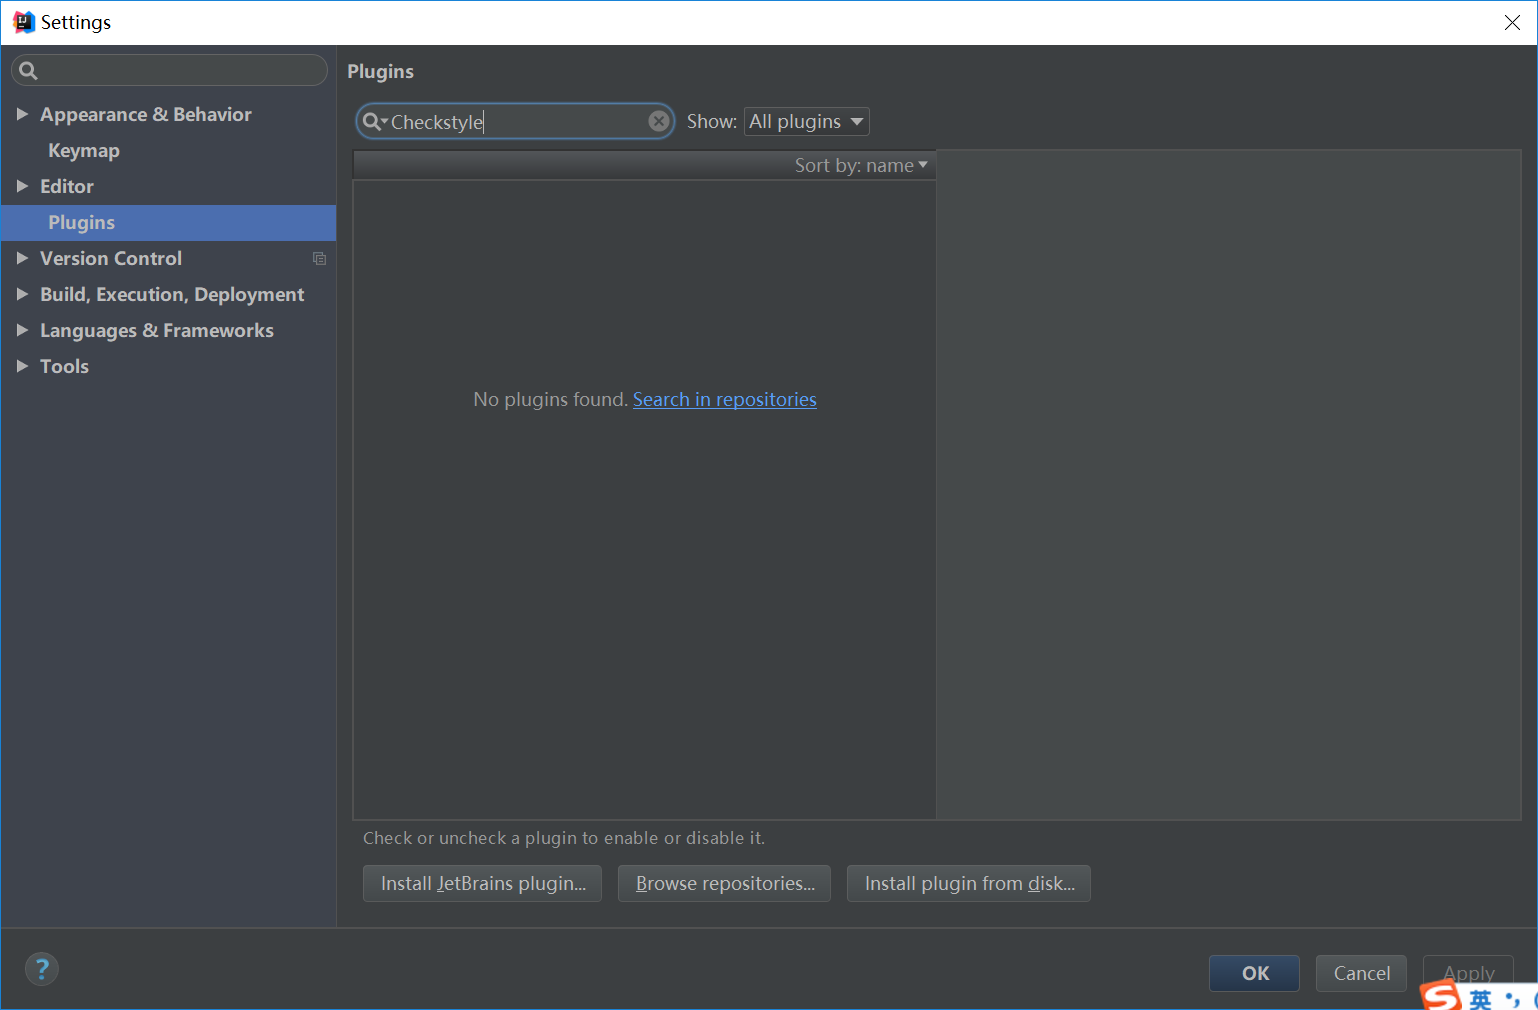
\includegraphics[width=12cm]{/../figures/cs-1}
\caption{Plugins选项卡}
\label{fig:cs-1}
\end{figure}

然后,点击其中的Search in repositories,在弹出的窗口中点击Install,如图\ref{fig:cs-2}所示。等待安装完成后,由此即完成了IntelliJ上Checkstyle的安装。

\begin{figure}
\centering
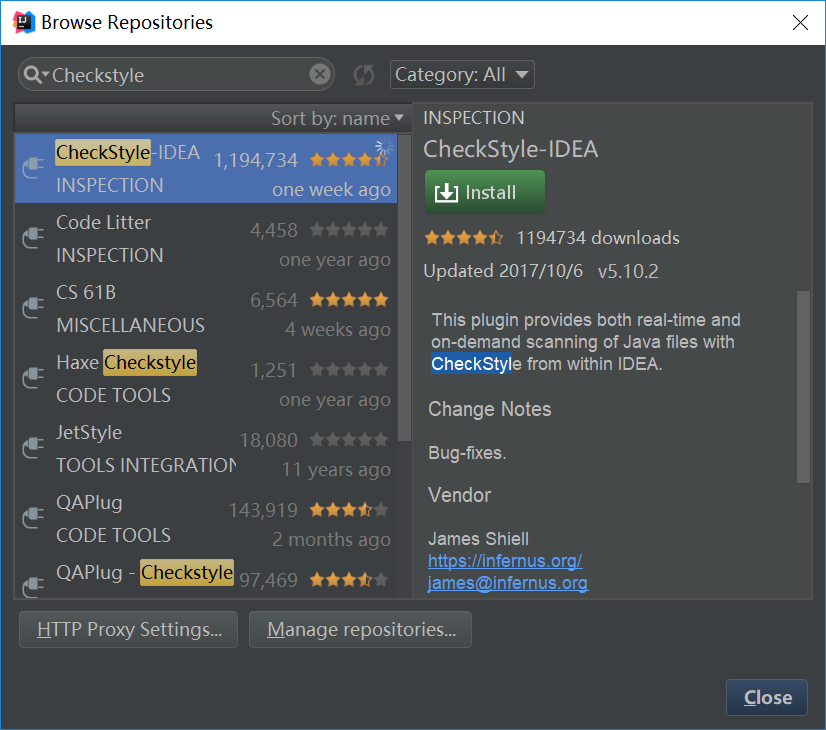
\includegraphics[width=10cm]{/../figures/cs-2}
\caption{Browse Repositories界面}
\label{fig:cs-2}
\end{figure}

在安装完成后,我们在Setting中左边栏选择Other Settings,Checkstyle。在出现的页面中的Configuration File选项中选择默认的Sun Checks作为风格检查的标准,如图\ref{fig:cs-3}所示,然后点击OK进行确定。由此,即完成了Checkstyle的配置。
\begin{figure}
\centering
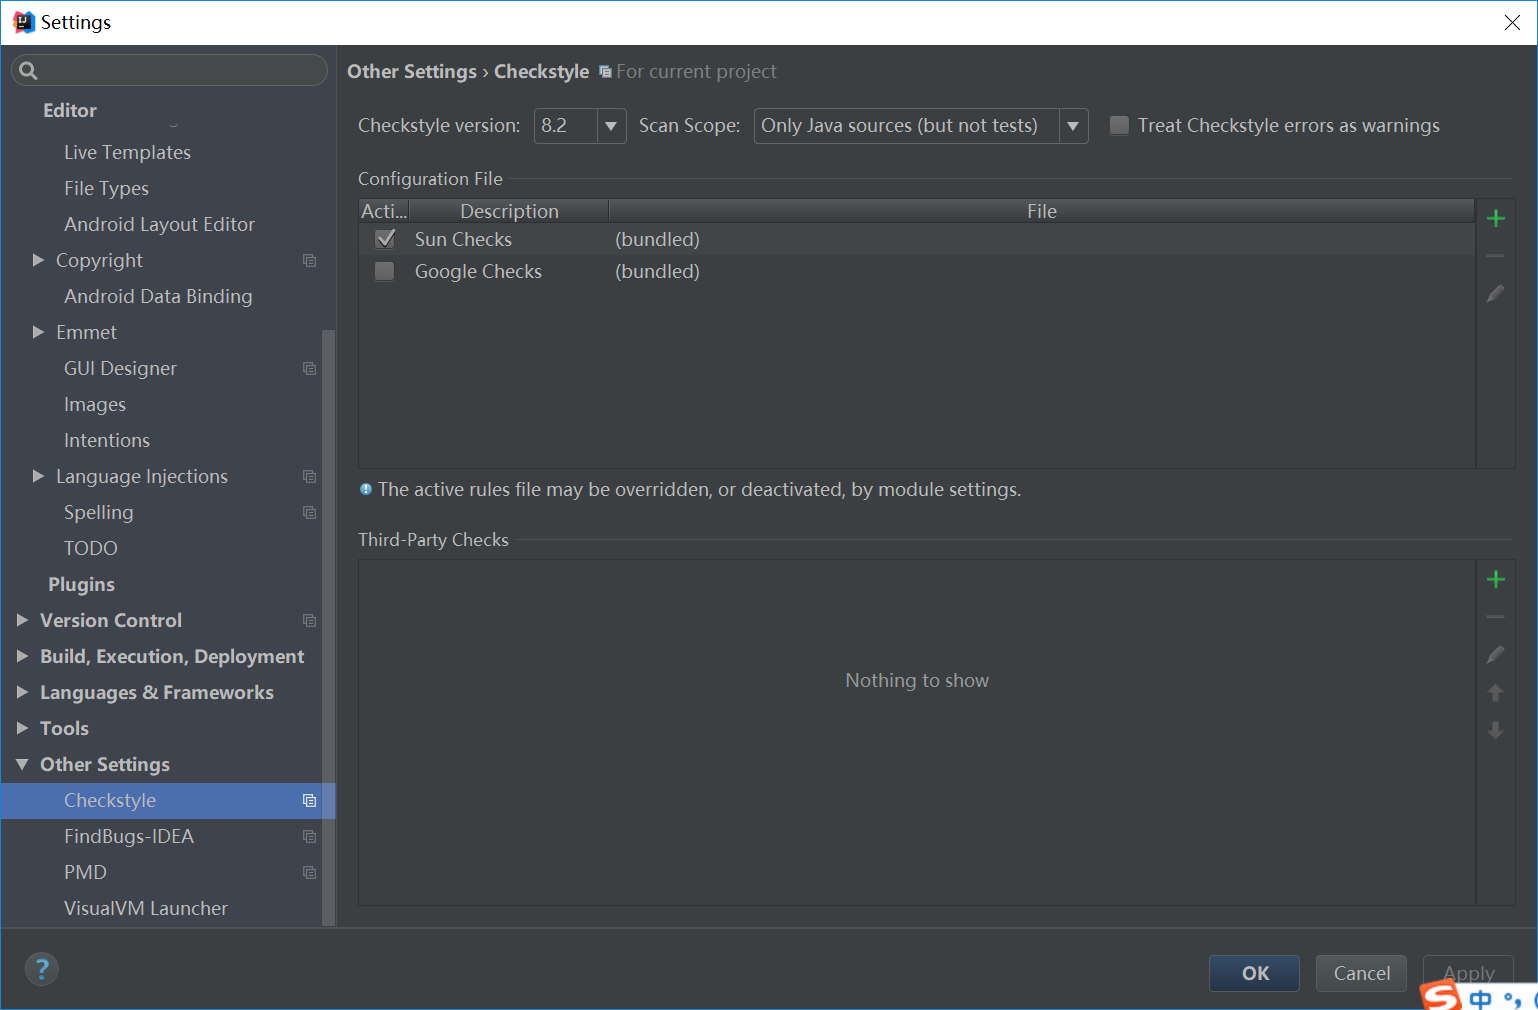
\includegraphics[width=12cm]{/../figures/cs-3}
\caption{设置检查标准}
\label{fig:cs-3}
\end{figure}

\BiSection{PMD}{}
在本节中,将描述在IntelliJ中安装以及配置PMD的方法。

与Checkstyle的安装方式基本一致,首先我们在Setting中的Plugins选项卡内输入“PMD”,点击Search in repositories,在出现的窗口中选择PMDPlugin,点击Install进行安装,等待安装完成。安装完后如图\ref{fig:pmd-1}所示。

\begin{figure}
\centering
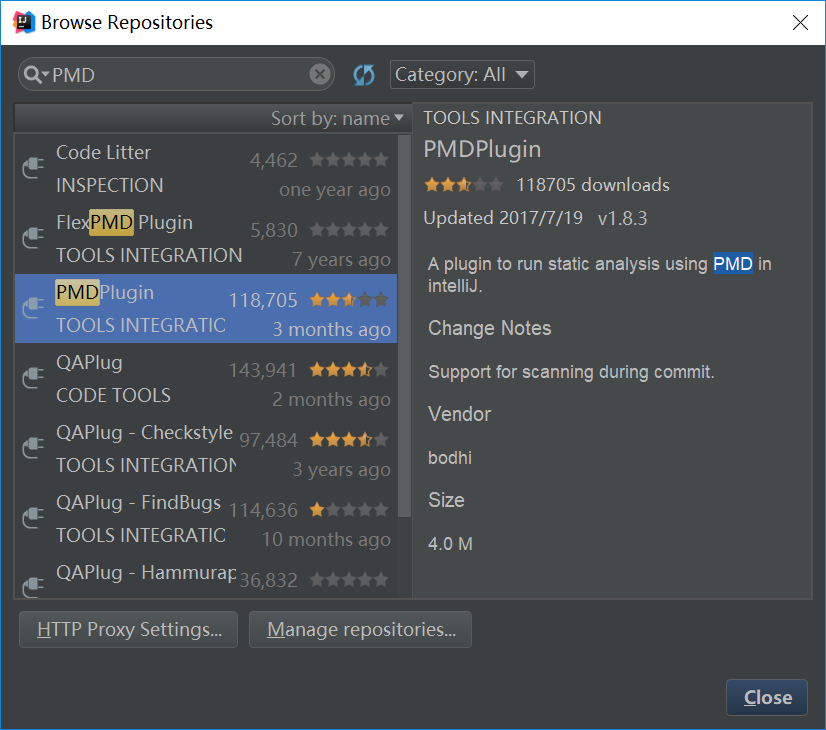
\includegraphics[width=10cm]{/../figures/pmd-1}
\caption{安装PMD}
\label{fig:pmd-1}
\end{figure}

由于本次实验中我们将直接使用PMD默认的配置,因此不需要进行额外的配置。

\BiSection{FindBugs}{}
在本节中,将描述在IntelliJ中安装FindBugs的方法。

与Checkstyle的安装方式基本一致,首先我们在Setting中的Plugins选项卡内输入“FindBugs”,点击Search in repositories,在出现的窗口中选择FindBugs-IDEA,点击Install进行安装,等待安装完成。安装完后如图\ref{fig:fb-1}所示。

\begin{figure}
\centering
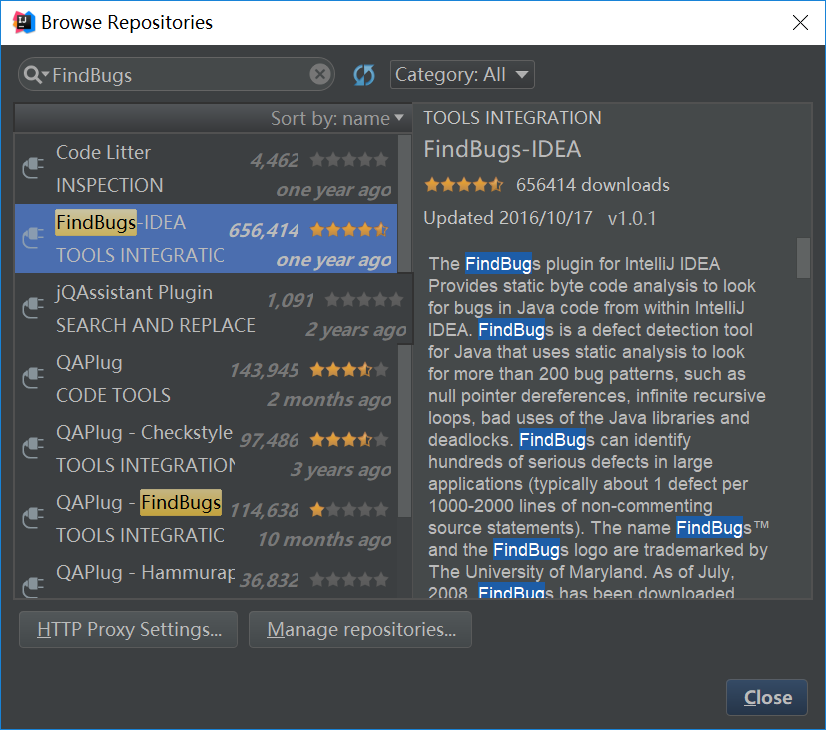
\includegraphics[width=10cm]{/../figures/fb-1}
\caption{安装FindBugs}
\label{fig:fb-1}
\end{figure}

\BiSection{VisualVM}{}
在本节中,将描述在IntelliJ中安装VisualVM的方法。

由于JDK中自带VisualVM软件,因此不需要额外安装VisualVM。不过,为了能够在IntelliJ中方便地使用VisualVM,我们选择安装VisualVM Launcher插件。该插件的安装过程与Checkstyle的安装方式基本一致,首先我们在Setting中的Plugins选项卡内输入“VisualVM”,点击Search in repositories,在出现的窗口中选择VisualVM Launcher,点击Install进行安装,等待安装完成。安装完后如图\ref{fig:vv-1}所示。

\begin{figure}
\centering
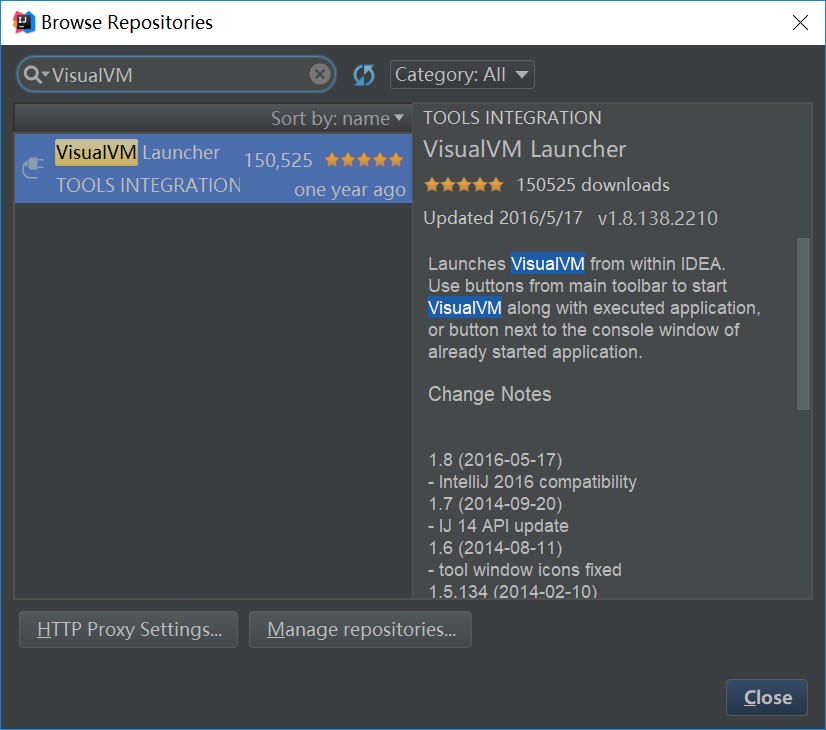
\includegraphics[width=10cm]{/../figures/vv-1}
\caption{VisualVM Launcher安装}
\label{fig:vv-1}
\end{figure}

% -------------------------------章节分割线-------------------------------
\BiChapter{本次实验所评审的代码}{}

% -------------------------------章节分割线-------------------------------
\BiChapter{代码review记录}{}

% -------------------------------章节分割线-------------------------------
\BiChapter{Checkstyle所发现的代码问题清单及原因分析}{}

% -------------------------------章节分割线-------------------------------
\BiChapter{PMD所发现的代码问题清单及原因分析}{}

% -------------------------------章节分割线-------------------------------
\BiChapter{FindBugs所发现的代码问题清单及原因分析}{}

% -------------------------------章节分割线-------------------------------
\BiChapter{VisualVM性能分析结果}{}
在本章中,将利用VisualVM工具对项目的执行时间以及内存占用情况进行分析,并根据分析得出的结果对项目代码进行改进。
最后将测试改进后的代码的执行时间以及内存占用情况,并与为改进之前的情况进行对比。

\BiSection{执行时间的统计结果与原因分析}{}
在本节中,将分别分析项目在生成与展示有向图,查询桥接词,根据桥接词生成新文本,计算两个单词之间的最短路径,以及随机游走这五个功能方面的耗时,并对耗时的原因进行分析。

需要说明的是,虽然在Lab1的原始要求中“读取并生成有向图”以及“展示有向图”为两个功能,但是在该项目中完成文件的读取以及有向图的生成后即自动展示了有向图,因此在此将原始要求中的两个功能需求合并为“读取并展示有向图”一个功能,并对这一个功能进行分析。

\BiSubsection{生成与展示有向图}{}
在生成与展示有向图的时间测试中,我们采用Lab1验收时的测试数据作为输入进行测试,耗时结果的统计见图\ref{fig:time-1}。

\begin{figure}
\centering
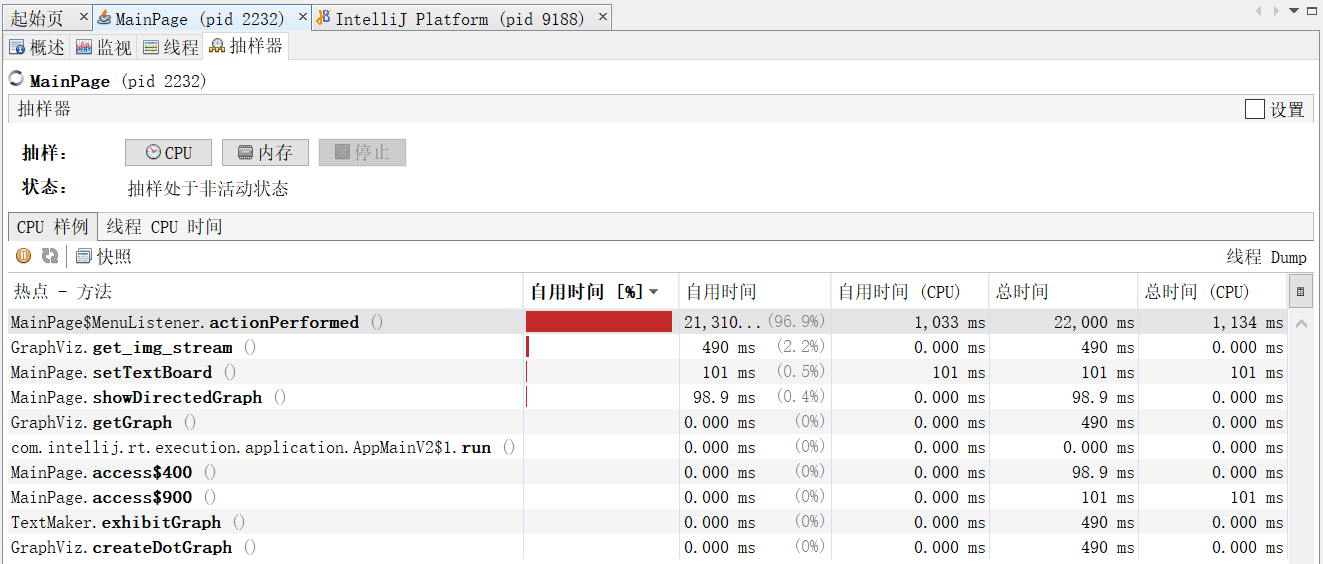
\includegraphics[width=12cm]{/../figures/time-1}
\caption{生成与展示有向图耗时}
\label{fig:time-1}
\end{figure}

需要首先特别说明的是,MenuListener.actionPerformed()的耗时为用户选择所要读取的文件时的耗时,因此不算在程序的运行时间内。在耗时图像中,Graphviz.get\_img\_stream()为调用外部程序Graphviz绘制图像,并从Graphviz读取其返回的图像的二进制串的函数,Graphviz.createDotGraph()为接受Graphviz源程序作为输入,并最终将生成的图片写入到文件中的函数,TextMaker.exhibitGraph()为生成程序中图的结构对应的Graphviz源程序,并最终将生成的图片写入到文件中的函数,MainPage.setTextBoard()为配置GUI左侧展示文本框的函数,MainPage.showDirectedGraph()为配置GUI中展示有向图部分的GUI元素的函数。

由此可见,除去用户操作的时间外,主要占用时间的函数为Graphviz.get\_img\_stream(),MainPage.setTextBoard(),以及MainPage.showDirectedGraph()这三个函数。

\BiSection{内存占用的统计结果与原因分析}{}
\BiSection{代码改进之后的执行时间统计结果}{}
\BiSection{代码改进之后的内存占用统计结果}{}

% -------------------------------章节分割线-------------------------------
\BiChapter{利用Git/GitHub进行协作的过程}{}

% -------------------------------章节分割线-------------------------------
\BiChapter{评述}{}
\BiSection{对代码规范方面的评述}{}
\BiSection{对代码性能方面的评述}{}

% -------------------------------章节分割线-------------------------------
\BiChapter{计划与实际进度}{}

% -------------------------------章节分割线-------------------------------
\BiChapter{小结}{}


%%% Local Variables:
%%% mode: latex
%%% TeX-master: "../main"
%%% End:
